In this chapter, we will address RQ1 based on the results obtained for each project.
The results will be shown visually using a \emph{historical graph}, a graphic representation that allows to easily identify the timespan for which commits we could built or not.
In addition, we will group the errors obtained from the logs when commits could not be built.

A summary with the results is shown in Table~\ref{table:allResults}.
This table offers, for each project, the total number of commits available in its history, the number of commits whose build succeeded, the number of commits whose build failed, the percentage of failures with respect to the total of commits, and the number of distinct syntoms (result of grouping identical errors).We can see that there is a project with hardly any errors (Closure Compiler). With the exception of the Apache Commons-math project, in the remaining projects, the failure rate exceeds 40\%. The Spring Framework project stands out not only for its size (it has a multitude of modules) and for its large number of commits, it also has a great variety of different symptoms detected that considerably enrich the later taxonomy.
The rest of this chapter presents a more detailed analysis for each of the projects.

\begin{table*}[h]
	\caption{Summary of experiments}
	\label{table:allResults}
	\begin{center}
	\begin{tabular}{crrrrr}
		\toprule
		\bf{Project} & \bf{\# commits} & \bf{\# success} & \bf{\# fails} & \bf{\% fail} & \bf{\# distinct syntoms}\\ 
		\midrule
		Closure Compiler & 2,858 & 2,855 & 3 & 0.10\% & 3\\
		Apache commons-lang & 3,570 & 1,897 & 1,673 & 46.86\% & 14\\
		Apache commons-math & 4,878 & 3,858 & 1,020 & 20.91\% & 18 \\
		Mockito & 2,639 & 538 & 2,101 & 79.61\% & 9 \\
		Joda-Time & 1,717 & 224 & 1,493 & 86.95\% & 1 \\
		Spring Framework & 17,382 & 6,013 & 11,070 & 63.68\% & 41\\
		\midrule
		Average & 5,507.3 & 2,524 & 2,983.3 & 50.20\% & 14,3 \\
		\bottomrule
	\end{tabular}
	\end{center}
\end{table*}

\section{Closure Compiler}

Our results show that the Closure Compiler project is a highly buildable project (Figure~\ref{fig:closureHist}) with 2,855 commits that can be built out of 2,858 (only 0.1\% of the builds failed).
Note that in the figure older commits appear on the left, with more recent commits on the right.
%Each column in the graph represents 100 commits. \grex{Maybe we should explain a little bit more the graph... I don't understand for instance why we have the white square for the most recent commits}\michel{An explanation of the graphics prior to the individual studies?}
Users of this project can rely on almost any previous snapshots being \emph{buildable}.
%The errors that occur are residual.

\begin{figure}[h]
	\begin{center}
		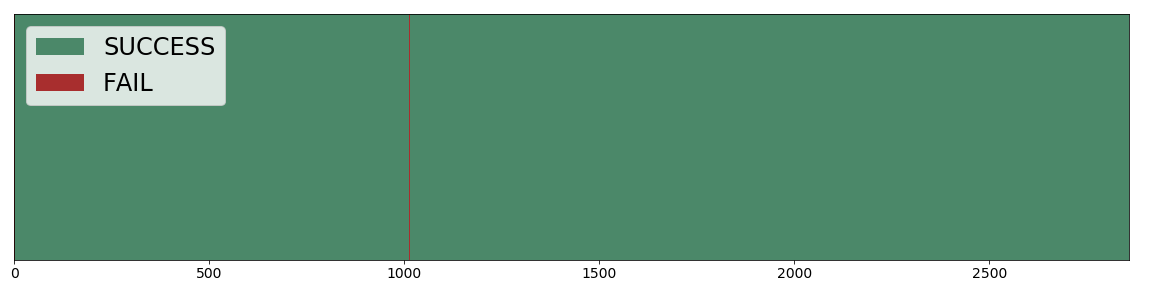
\includegraphics[width=\linewidth]{charts/ClosureHist}
		\caption{Build history of Closure Compiler project}
		\label{fig:closureHist}
	\end{center}
\end{figure}

\section{Apache commons-lang}

\begin{table}[h]
	\caption{Grouped errors in Commons-lang builds}
	\label{table:langErrors}
	\begin{center}
	\begin{tabular}{lr}
		\toprule
		\bf{Error} & \bf{count} \\ 
		\midrule
		There is no POM in this directory & 1,524 \\
		Unmappable character for encoding UTF8	& 110 \\
		error: cannot find symbol in NullComparator.java & 20 \\
		Non-resolvable parent POM & 5 \\
		error: cannot find symbol in UnicodeUnescaper.java & 2 \\
		IDKey is not public in org.apache.commons.lang & 2 \\
		Error: variable options might not have been initialized & 2 \\
		Error: incompatible types & 2 \\
		Others & 6 \\
		\bottomrule
	\end{tabular}
	\end{center}
\end{table}

%\grex{I see some of the errors begin with ``Error: '', others don't. Could we have families of higher-level errors?}

In this project we can observe a consistent build failure starting around the middle of the history (Figure~\ref{fig:langHist}).
In this case, we obtain a failure rate that reaches almost half of the project (46.86\%).
The errors collected for this project are shown in Table~\ref{table:langErrors}.

\begin{figure}[h]
	\begin{center}
		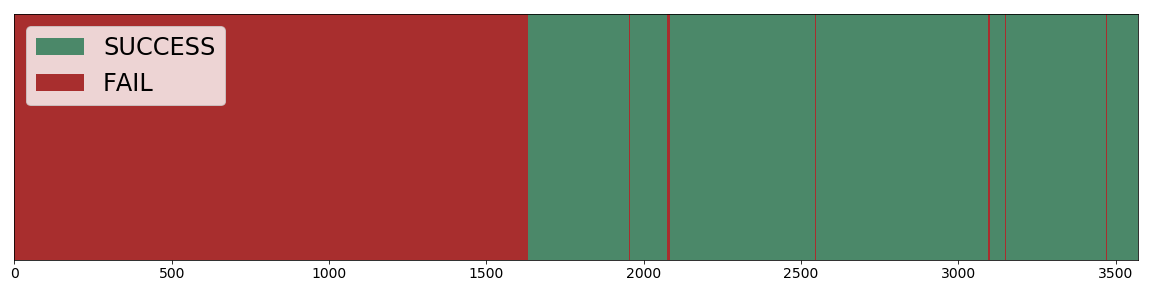
\includegraphics[width=\linewidth]{charts/LangHist}
		\caption{Build history of Apache Commons-lang project}
		\label{fig:langHist}
	\end{center}
\end{figure}

The main error of this project is the absence of the \textit{pom.xml} \emph{config} file, which is used by the maven build system to build the application.
When we looked into this, it was clear that this happened because the build system changed at some point; the project stopped using Ant to start using Maven.

\section{Apache commons-math}

The Math project is a robust one (Figure~\ref{fig:mathHist}), with a low failure rate (20.91\%).
Similar to the commons-lang project, there is a specific commit from which the builds begin to fail.
The errors collected are shown in Table~\ref{table:mathErrors}.

\begin{figure}[h]
	\begin{center}
		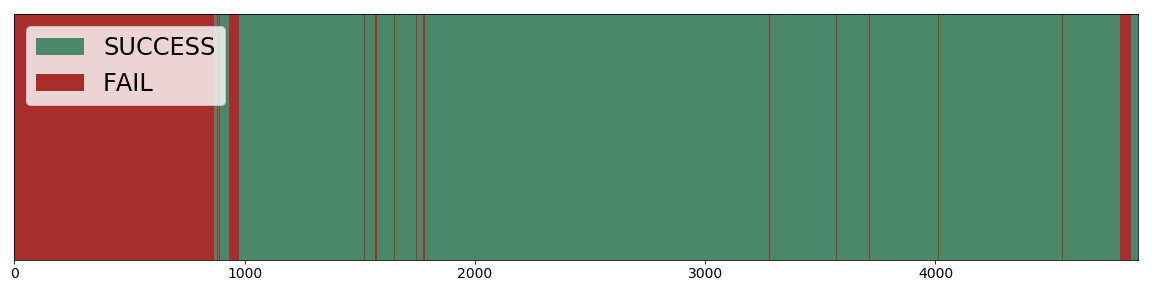
\includegraphics[width=\linewidth]{charts/MathHist}
		\caption{Build history of Apache Commons-math project}
		\label{fig:mathHist}
	\end{center}
\end{figure}


As in the Lang project, the build system for the project was changed, from Ant to Maven, which causes any build to fail in the most recent commits of the project.

\begin{table}[h]
	\caption{Grouped errors in Commons-math builds}
	\label{table:mathErrors}
	\begin{center}
	\begin{tabular}{lr}
		\toprule
		\bf{Error} & \bf{count} \\ 
		\midrule
		Can't read pom.xml: No such file or directory & 866 \\
		Failed to execute goal jacoco-maven-plugin & 52 \\
		Failed to execute goal cobertura-maven-plugin & 43 \\
		Error: cannot find symbol & 28 \\
		Failed to execute goal maven-compiler-plugin & 10 \\
		error: no suitable method found & 4 \\
		error: data has private access in ArrayFieldVector & 2 \\
		error: cannot assign a value to final variable entries & 2 \\
		error: Java name clash, have the same erasure & 2 \\
		error: SparseRealMatrix is not abstract & 2 \\
		error: LUDecompositionImpl is not abstract & 2 \\
		Others & 7 \\
		\bottomrule
	\end{tabular}
	\end{center}
\end{table}

\section{Mockito}

This project shows a very low buildability.
Most of its history commits (see Figure~\ref{fig:mockitoHist}) cannot be built.

\begin{figure}[h]
	\begin{center}
		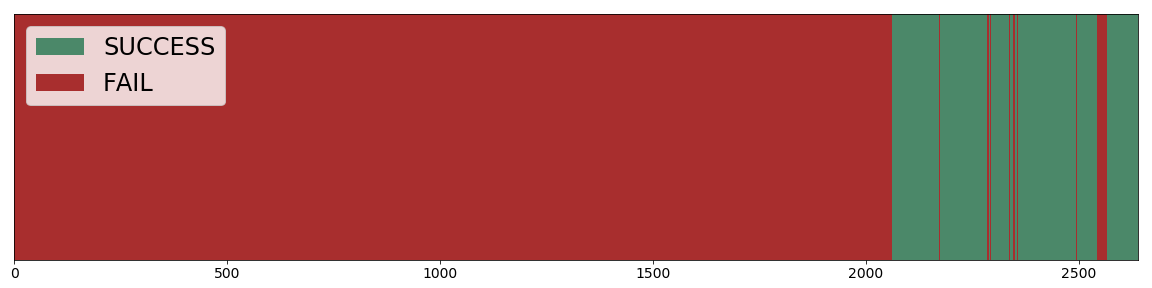
\includegraphics[width=\linewidth]{charts/MockitoHist}
		\caption{Build history of Mockito project}
		\label{fig:mockitoHist}
	\end{center}
\end{figure}

\begin{table}
	\caption{Grouped errors in Mockito builds}
	\label{table:mockitoErrors}
	\begin{center}
	\begin{tabular}{lr}
		\toprule
		\bf{Error} & \bf{count} \\ 
		\midrule
			gradlew: No such file or directory & 1,622 \\
			can't read buildSrc/build.gradle: No such file or directory & 440 \\
			Could not find net.bytebuddy:byte-buddy:0.2.0. & 14 \\
			A problem occurred evaluating script & 9 \\
			Execution failed for task ':jar'. & 6 \\
			Execution failed for task ':compileGroovy'.& 4 \\
			Execution failed for task ':compileJava'. &	3 \\
			unable to resolve class ReleaseNotesServices & 2 \\
			Others & 1 \\
		\bottomrule
	\end{tabular}
	\end{center}
\end{table}

The analysis of errors (Table~\ref{table:mockitoErrors}) shows that the main error found is that the \emph{gradlew} executable does not exist, due to a change in build system from Ant a Gradle.
Another very repeated error is the non-location of the build.gradle file, that was moved at some point to a different folder.


\section{Joda-time}

In this case (see Figure~\ref{fig:timeHist}), we found a high percentage of failures (86.95\%) that, in all cases, are due to a change of the build system, from Ant to Maven.

\begin{figure}[h]
	\begin{center}
		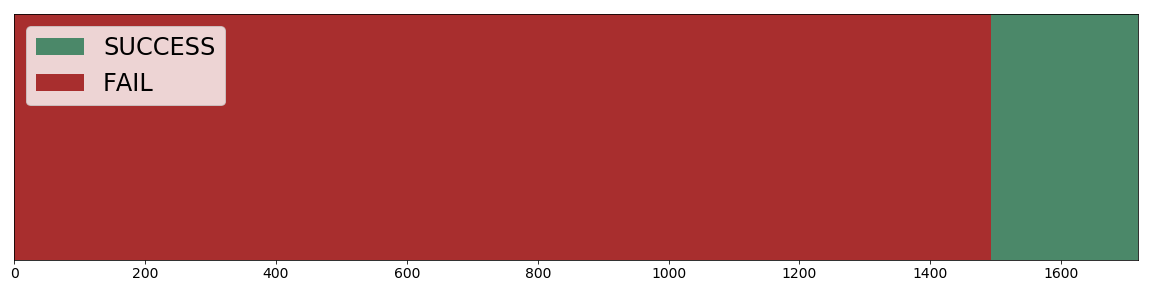
\includegraphics[width=\linewidth]{charts/TimeHist}
		\caption{Build history of Joda-time project}
		\label{fig:timeHist}
	\end{center}
\end{figure}

\section{Spring Framework}

This project is, by far, the one that contains more commits, which gives us a broader vision of how a more complex project behaves.
Just over two-thirds of the project's history (as shown in Figure~\ref{fig:springHist}) cannot be built.
There is a consecutive set of commits where it becomes more buildable.
Finally, in the more recent versions of the project, it is again difficult to find buildable commits.

\begin{figure}[h]
	\begin{center}
		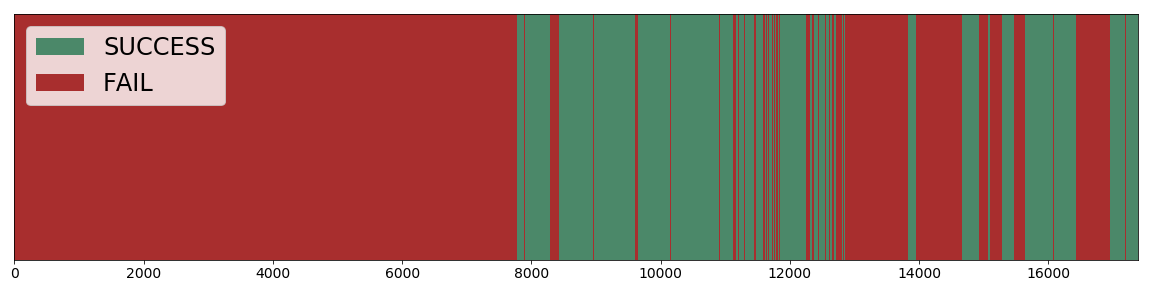
\includegraphics[width=\linewidth]{charts/spring-frameworkHist}
		\caption{Build history of Spring Framework project}
		\label{fig:springHist}
	\end{center}
\end{figure}

\begin{table}
	\caption{Grouped errors in Spring Framework builds}
	\label{table:springErrors}
	\begin{center}
	\begin{tabular}{lr}
		\toprule
		\bf{Error} & \bf{count} \\ 
		\midrule
		gradlew: No such file or directory& 5633  \\
		Cannot allocate memory & 2353  \\
		Invalid byte tag in constant pool & 470   \\
		Could not find group:com.itextpdf & 460   \\
		The import java.util.Arrays cannot be resolved & 398   \\
		error: warnings found and -Werror specified 1 error & 328   \\
		Bad file descriptor & 299   \\
		error: cannot find symbol & 218   \\
		error: incompatible types & 210   \\
		Could not determine which tasks to execute  & 206   \\
		error: unmappable character for encoding ASCII  & 202   \\
		Could not resolve all dependencies for spring-webmvc:optional & 132   \\
		error: constructor (..) cannot be applied to given types & 80 \\
		Execution failed for task ':spring-asm:compileJava'. & 77    \\
		error: constructor (..) cannot be applied to given types & 72    \\
		error: EmbeddedDataSourceProxy is not abstract & 64    \\
		FileNotFoundException & 41    \\
		error: package javafx.application does not exist & 28    \\
		Could not resolve all files for configuration ':classpath'. & 25    \\
		Could not find reactor-net:1.1.0.BUILD-SNAPSHOT. & 19    \\
		Could not find reactor-core:1.0.0.BUILD-SNAPSHOT. & 10    \\
		A problem occurred evaluating root project 'spring' & 9 \\
		error: no suitable method found & 6 \\
		A problem occurred evaluating root project 'spring' & 6     \\
		error: local variable (..) is accessed from within inner class & 3     \\
		error: GenericApplicationContext is not abstract & 3     \\                                                                       
		error: invalid method declaration; return type required & 2  \\
		error: package (..) does not exist & 2 \\    
		Others & 10 \\
		\bottomrule
	\end{tabular}
	\end{center}
\end{table}

As can be seen in Table \ref{table:springErrors}, the number of different errors for this project is far above any other of the studied projects.
The most common error is once again due to a change in the build system, from Ant to Gradle.
Other problems, derived from being a heavy and complex project, are the lack of memory to run the builds and the problem of downloading old or outdated libraries.

\vspace{0.3cm}
\begin{tcolorbox}[fonttitle=\bfseries,title=Answer to RQ1: Can we build all snapshots of a project?,label=rq1,colframe=blue!50!black]
	There are many parts of the history of projects that are not buildable.
	Despite Java being an static typed language, with well-known build systems, four out of six projects have build problems in more than 40\% of their commits.
\end{tcolorbox}









